\label{ch:results_model}

\subsection{Results}

\subsubsection*{Global visitation}
The sum of visits are not evenly distributed for all frequency stages (Fig.~\ref{fig:SUM}). A strong cover-dependent pattern is visible for small cluster values. The visits have a u-shaped relationship for 5\% cover and a fourth-degree polynomial function for higher cover values. The visitation drops to a minimum at 90:10 ratio and peaks again for balanced frequencies. Cluster reduce the frequency dependence. 

Note that the absolute visitation numbers vary additional to the shape for cover and cluster values. Both parameters have a frequency independent influence on the visitation rate (supplementary material, fig.~\ref{fig:nonfreq}). Floral cover shows a Holling´s type II functional response saturated at 30\% and the visits for degree of clustering have a hump-shaped relationship with a peak at an intermediate agglomeration level of 5-10 flowers per cluster.

\subsubsection*{Per-flower visitation rate}
The per-flower visitation shows a similar cubic function as the data collected in the Jena Experiment (Fig.~\ref{fig:PFV}A,B). Within the first 20\% there is a steep increase in visits per flower. Afterwards, additional gain of visits is for all cover values above 5\% not proportional with the increase of flowers due to higher frequency, the per-flower visitation drops with a minimum around 80\%. Towards 100\%, when the species gets exclusive, the per-flower visitation rises again. 
Cover and cluster both influence the frequency dependence. The higher the cover, the lower the per-flower visitation and the bigger the cluster the less visible is the frequency dependence. Simulations with more than 10 flowers per cluster show a high variance for frequencies below 10\% and very low to no frequency dependence afterwards (Fig.~\ref{fig:PFV}C,D). 

The same data is plotted as proportion of visits to species A to take the variance in the sum of visits into account (Fig.~\ref{fig:PFV}E-H; see previous section "Global visitation"). It shows a clear negative frequency dependence favoring the rare specie. Below 50\%,species A gets more visits than would be proportional, above 50\% the curve is mirrored because both species are identical in the simulation and the common species gets unproportional few visits. The higher the cover, the stronger is the frequency dependence. For higher cluster values, all data points approach a frequency independent relationship (Fig.~\ref{fig:PFV}H). 

\subsubsection*{Pollination ratio}
The pollen-carryover rate is defined as maximum number of visits within a successful pollination can take place. In the model, I tested values from 1 (strong heterospecific pollen interference) to 16 (weak heterospecific pollen interference). Figure~\ref{fig:POC} gives the proportion of all visits where a successful pollination took place. The first 20\% frequency are crucial for all parameter-value combination. A very steep increase up to 80\% successful pollinated flowers is followed by a moderate linear increase up to 100\% for exclusive existence. The pollen-carryover rate only makes a difference for small cover and cluster values (Fig.~\ref{fig:POC}a). The higher the cover and the bigger the cluster, the better is also the proportion of successful pollination, even for small frequencies, independent of the pollen-carryover rate(Fig.~\ref{fig:POC}c,f,g-i). 

\subsection*{Sensitivity analysis}
Aim of the sensitivity analysis is the understanding of the underlying behavior parameters on the outcome of the model. Therefore, pollinator density, reward regrowth, search time and vision were tested for a (unnaturally) broad range of values and analyzed as proportional data to check for difference to the empirically founded default values. Vision, search time and the number of bees on the meadow influence the sum of visits (Fig.~\ref{fig:SA_SUM}). A higher vision leads to more visits in a saturated curve, the search limit reduces the number of visits and more bees lead again to more visits per time unit. The reward function has only for a very high regrowth rate an small negative influence on the total number of visits.

\subsubsection*{Reward regrowth}
Only a considerably high regrowth rate (0.1J/sec, yellow line in fig.~\ref{fig:SA_reward}) has a reversing effect on the frequency dependence: Rare species get unproportionally few visits whereas common species benefit from a positive frequency dependence. The influence is less severe with increasing cluster size. 

% Hence, a high reward can fix decrease diversity
% with very high reward rates, the bees find rarely a flower with bad reward and are changing preference less often. The only other way of changing preference is unsuccessful flight and that favors the common species
%IMPORTANT! Explained all lab experiments dome by smithson et al 1997a,1997b & 1996

\subsubsection*{Pollinator vision distance}
Every bee-agent can detect flowers in a 180$^{\circ}$ cone-shaped array of patches to their front. The number of patches in that array is determined by the vision distance. A high vision increases the sigmoid frequency dependence even in a heavily clustered model environment (Fig.~\ref{fig:SA_view}). If the bee-agents are only able to see the direct neighbor, the frequency dependence is reversed to favor the common species for low cluster values. 

%with high vision bee-agents are able to detect flowers of the rare species more quickly and are less likely to change their preference
%similar result as changing search time limit or make density higher
%if the bee can see further it will fly more directly to the next flower without too much random walk. but on the other hand it will fly for longer distances instead of changing preference to the more abundant species. Less efficient, less total visits

\subsubsection*{Search time limit}
If a bee-agent searches longer than a given search time limit unsuccessfully for a unvisited and preferred flower, the probability to switch preferences will increase by 10\% with every additional step. The search limit was altered from 1 to 50 seconds in the sensitivity analysis. The results are similar to the effect of vision as they also change the probability to switch preferences. Higher search time limits lead to stronger negative frequency dependence benefiting the rare species. A search limit of 1 second reduces the dependency (Fig.~\ref{fig:SA_flight}).

%with higher search time limit, the bee continues to search for the rare species instead of changing to the more abundant species. That is less efficient (less absolut visits) and enhances the FD
 
\subsubsection*{Pollinator density}
Besides the expected increase of absolute visits, a change of pollinator density has no effect on the outcome of the model at any cover or cluster values (Fig.~\ref{fig:SA_bees}).

\begin{figure} [h] %results:SUM
	\centering
	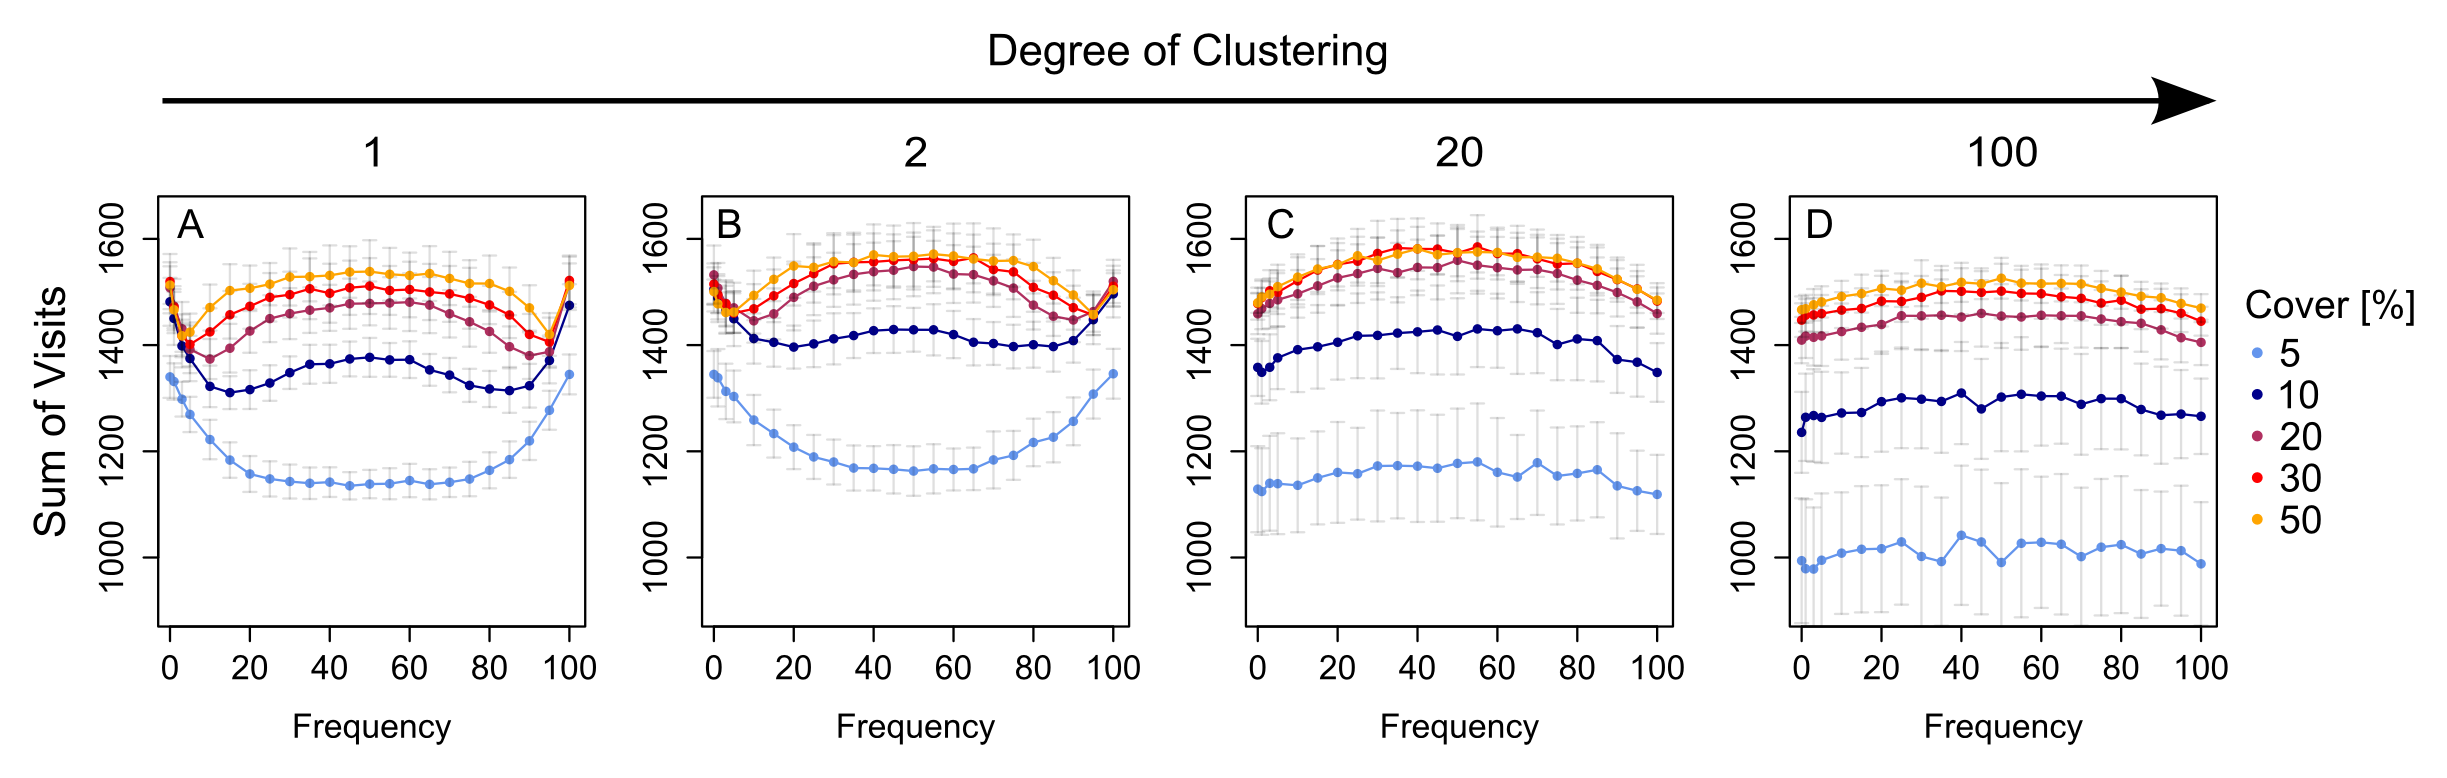
\includegraphics[width=17cm]{Images/SUM}
	\caption{Summed visits to both species show a frequency dependence for low cluster values. Depending on the floral cover it is quadratic or a fourth-degree polynomial relationship. Maximum of visits (maximal efficiency) is achieved for very unequal or very equal frequencies. If one species is rare, the sum of visits drop because some bee-agents forage inefficiently on the rare species, having long flight and searching times. Clustering reduces the frequency dependence but also decreases the absolute number of visits and increases the variance (grey error bars).}
	\label{fig:SUM}
\end{figure}

\begin{figure} [ht] %results:PFV
	\centering
	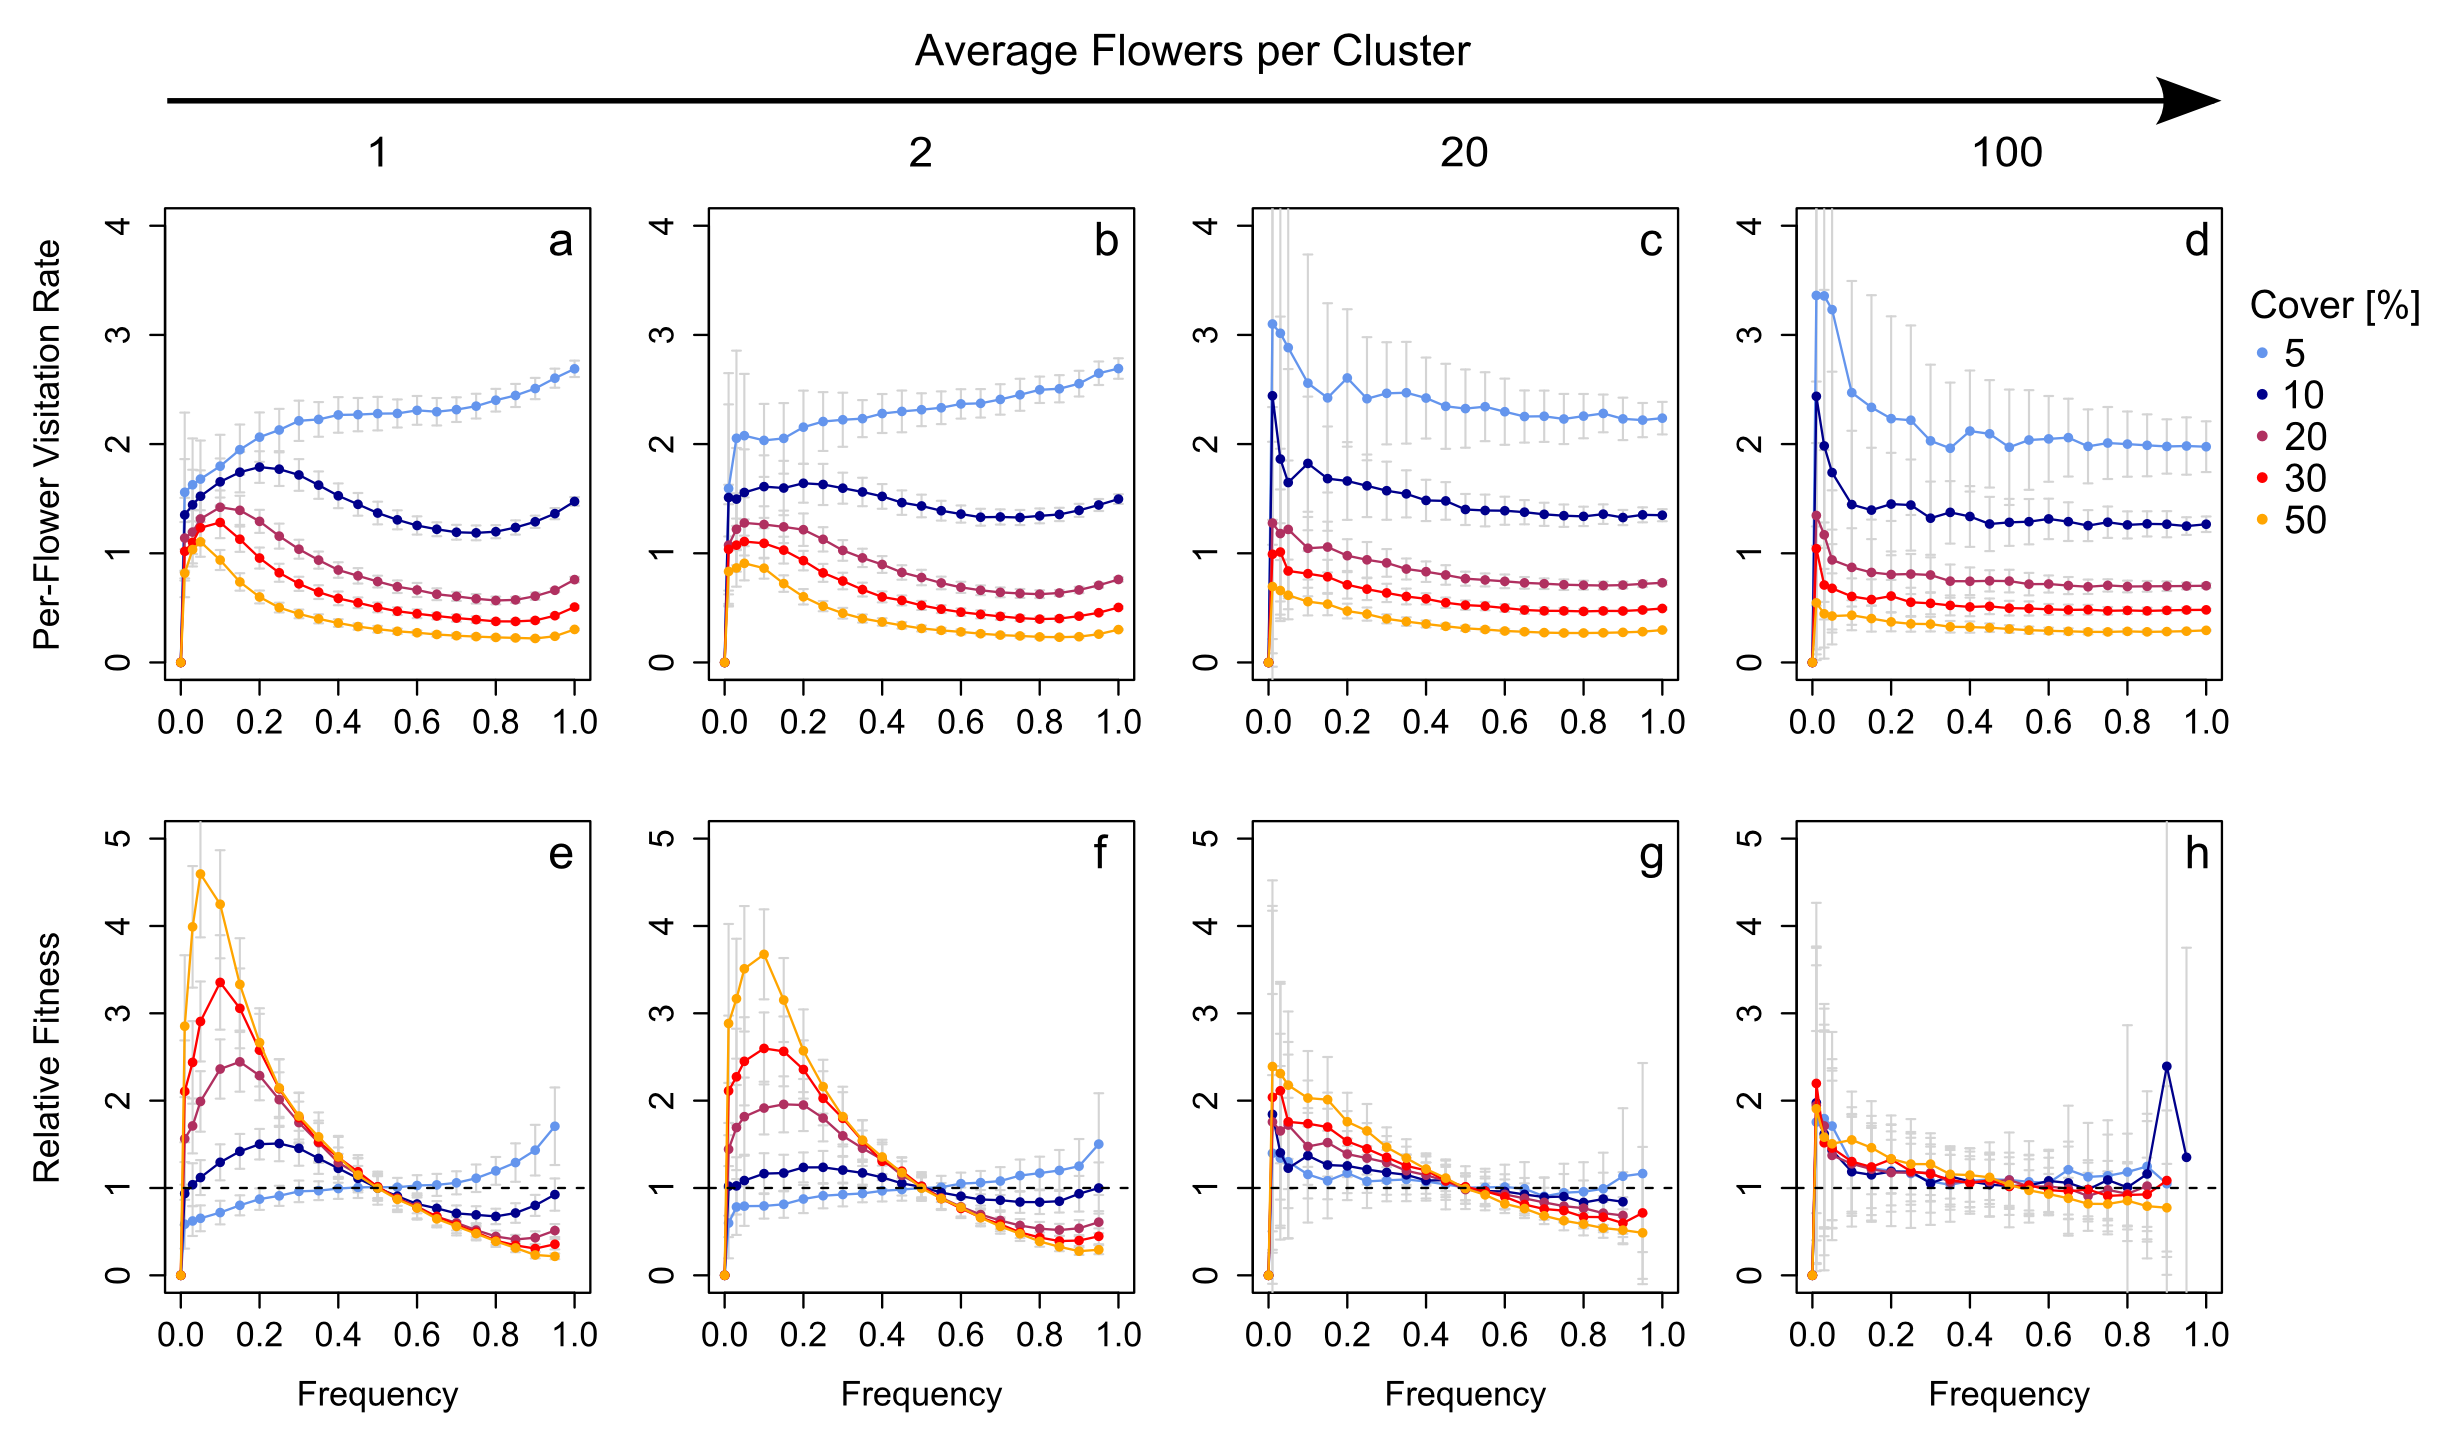
\includegraphics[width=17cm]{Images/PFV}
	\caption{The main analysis of the agent-based model confirm the findings of the linear mixed effect model of the field data: The per-flower visitation rate shows a clear frequency dependence with a cubic relationship. Visitation rates increase within the first 10-20\% of frequency towards a maximum. For intermediate frequencies is the increase of flowers not proportional with additional visits. The per-flower visitation rate only increases again towards exclusiveness of the species. The effect is stronger for higher floral cover (2a-d). Increase in clustering reduces the frequency dependence (1d,2d).}
	\label{fig:PFV}
\end{figure}

\begin{figure} [ht] %results:POC
	\centering
	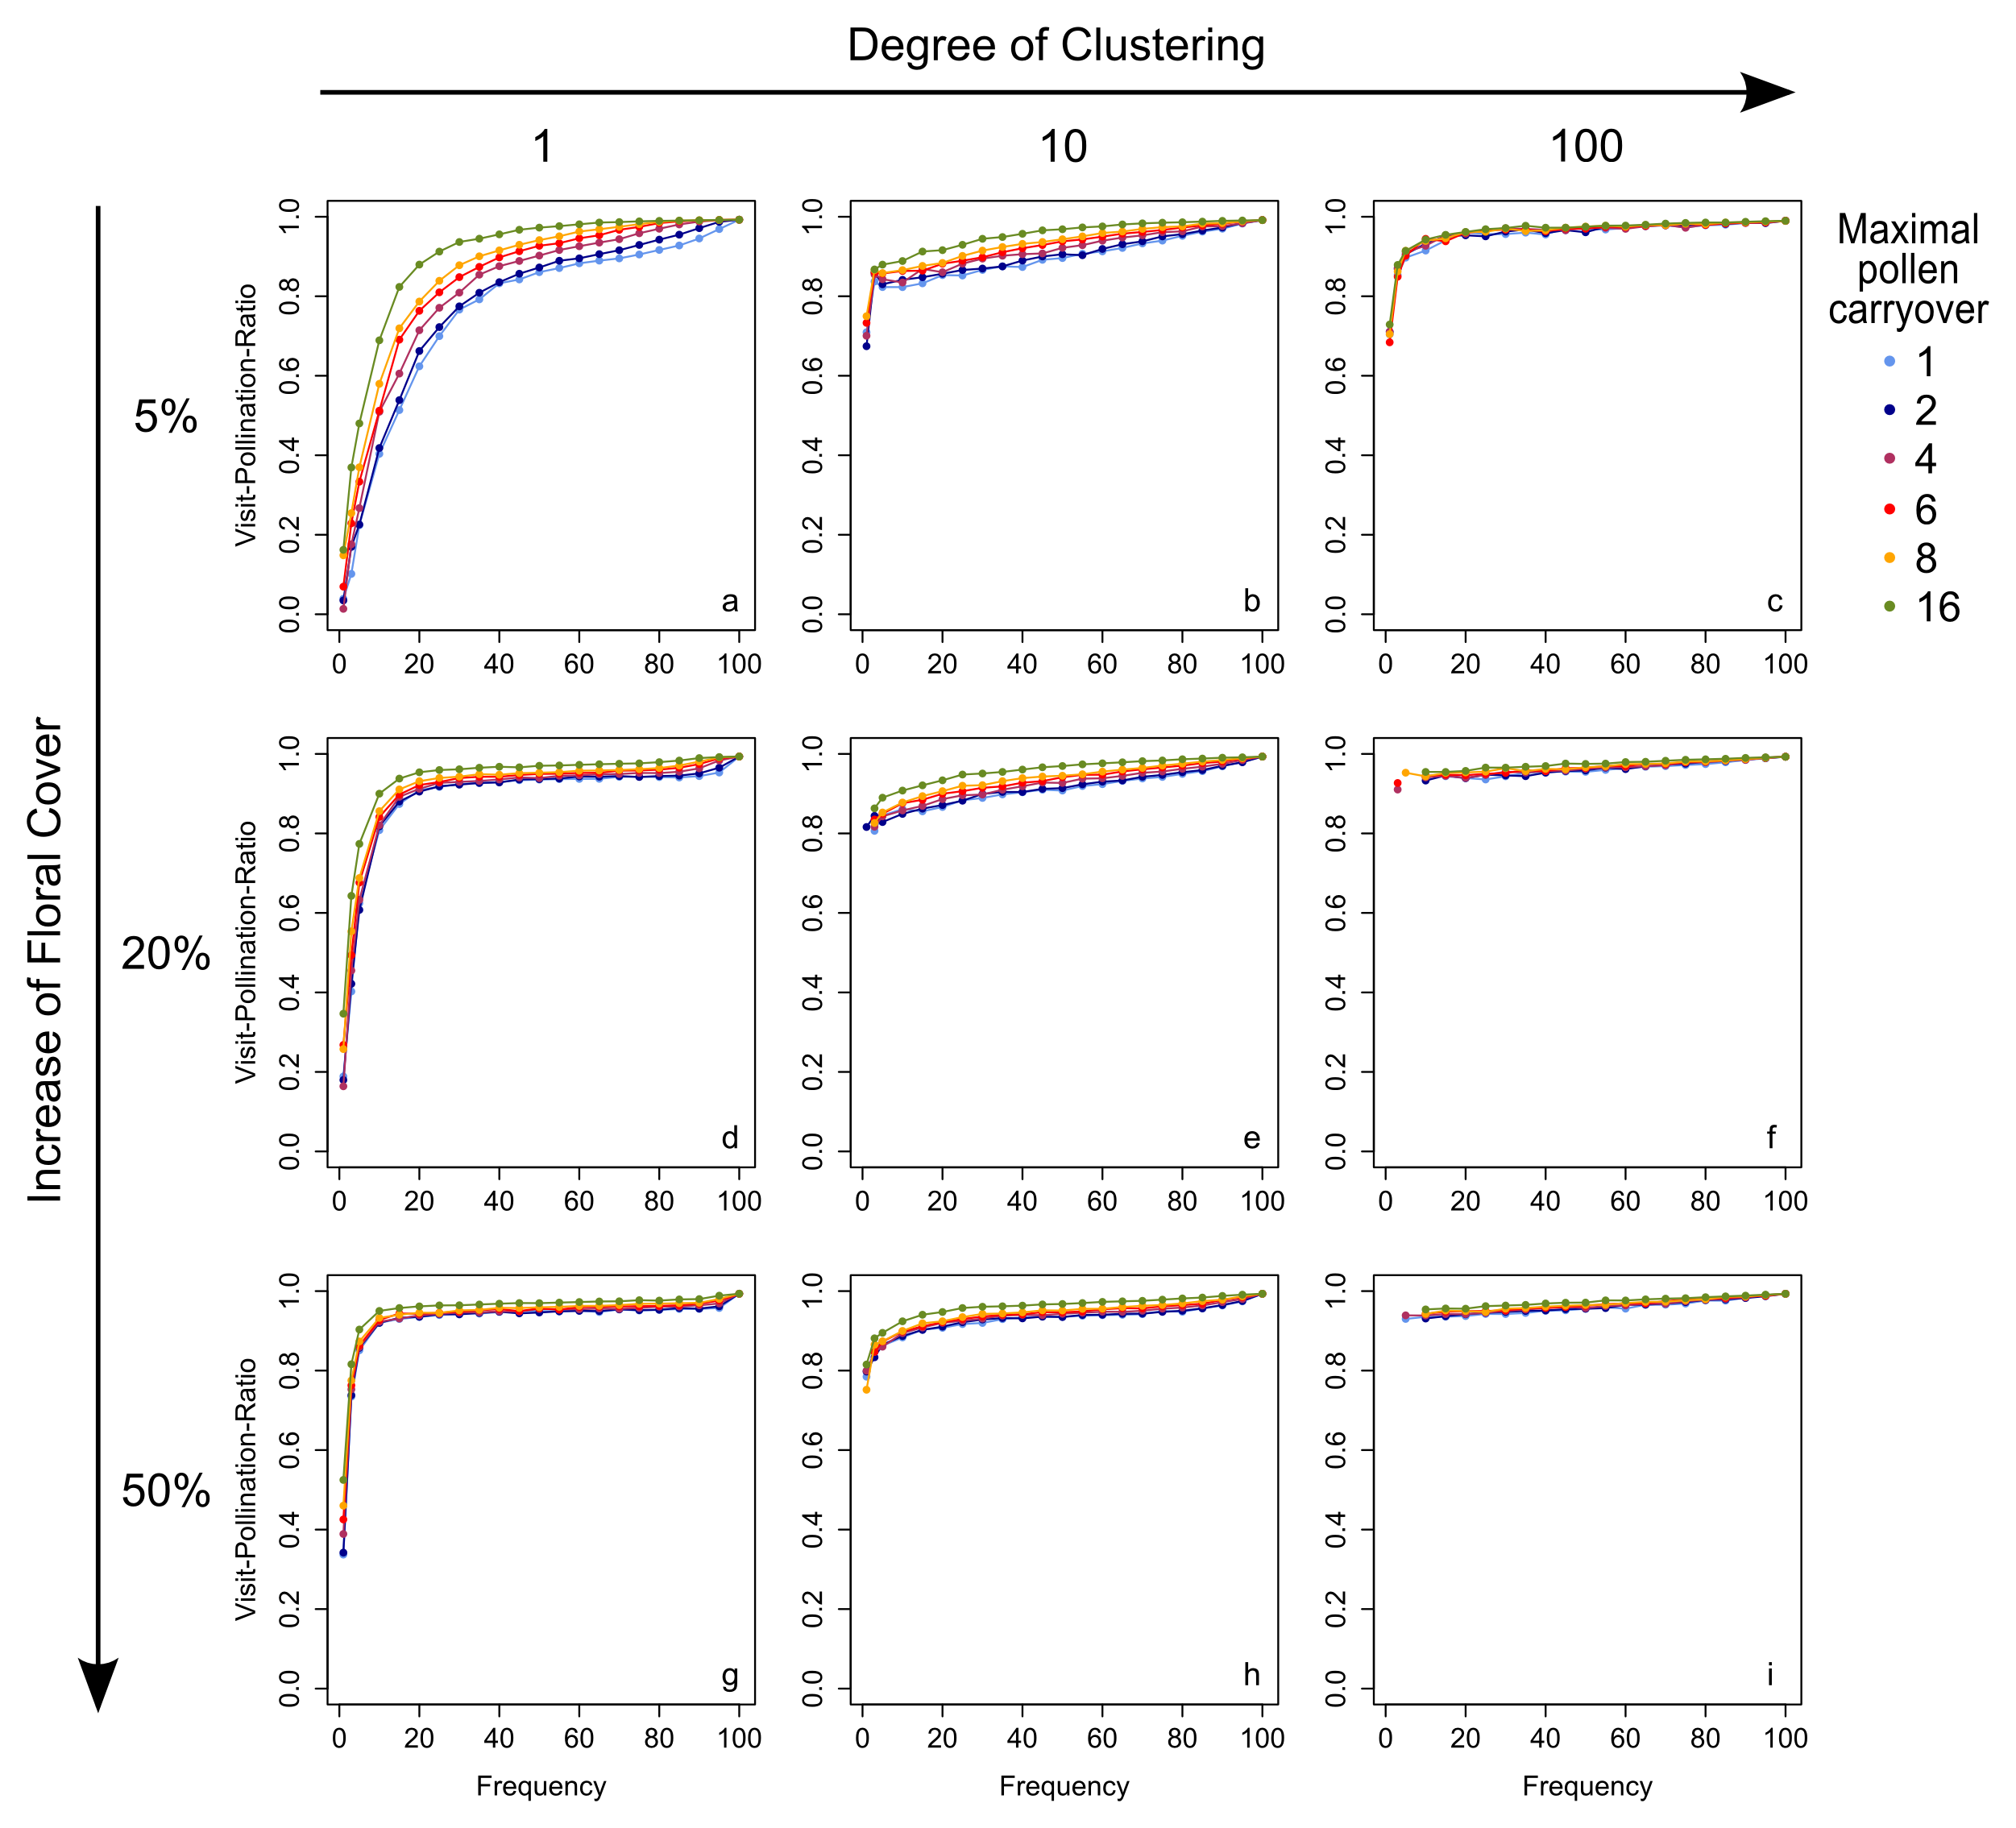
\includegraphics[width=17cm]{Images/POC}
	\caption{The pollen-carryover rate defines the maximum number of visits within a successful pollination is possible. With a pollen-carryover rate of one, the pollen can only be carried to the next flower. Therefore, the ratio of successful pollinations per visit can be seen as indicator for flower constancy \citep{montgomery2009pollen}. A high pollen-carryover rate is only important for a low cover and no-cluster environment. With increasing cover and cluster, the ratio becomes steeper for low frequencies which stands for more qualitative visits.}
	\label{fig:POC}
\end{figure}